% 0403 修改要点
% 1. 原图1 更换实物图、更换风格、对比度,放到method部分
% 2. 新的图1,典型结构的电路图
% 3. introduction 第二段 RBS 修改(增加的典型结构),列点的形式说明亮点,其余以删除为主
% 4. method 部分,最开始添一小段,结合原图1介绍流程
% 5. 第3 section 标题直接改为 examples,只包含:一个详细的结构、不同规模的对比、不同结构的对比,删去展望部分;修改图例,改善图的表示
% 6. conclusion 重写,包含展望
% 7. 全文主语的修改,逐段润色,caption的修改
% 8. abstract 修改
% 9. 转为 word



\documentclass{article}
\usepackage{graphicx}
\usepackage{subcaption}
\usepackage{enumerate}
\usepackage{amsmath}
\usepackage{multirow}
\usepackage{bm}
\usepackage[ruled,linesnumbered]{algorithm2e}

\def\T{\mathrm{T}}


\title{Greedy-based RBS maximum allowable current calculation method}
\author{3057761608 }
\date{March 2023}

\begin{document}

\maketitle

\begin{abstract}
    Traditional battery systems are limited by their dependence on the worst-performing battery cell, which negatively impacts their performance and lifespan.
    To overcome this limitation, Reconfigurable Battery Systems (RBSs) have emerged as a promising alternative, with the ability to dynamically adjust the circuit configuration to optimize the charging and discharging strategies of battery cells.
    However, due to their reconfigurability, RBSs require new performance indicators to evaluate their performance.
    This paper proposes an approach to estimate the Maximum Allowable Current (MAC), which is a crucial indicator for evaluating or optimizing the performance of RBSs.
    The proposed method utilizes a greedy algorithm based on a graph model and an equivalent circuit model.
    By searching for the shortest path for battery cells to connect to the main circuit in the graph model, a greedy search strategy is provided for the equivalent circuit model to describe the switch state variables.
    We validate the effectiveness of the proposed method on RBS structures of different sizes and configurations.
    Our results also show that the ratio of the output current to the maximum battery current could better reflect the structural performance of RBS than the output current alone.
\end{abstract}

\section{Introduction}

Battery Energy Storage Systems (BESSs) are widely used to store and supply high-quality electrical energy in various applications, including electric vehicles and wind power turbines\cite{desiqueiraControlStrategySmooth2021,karandehTwoStageAlgorithmOptimal2019,yangBatteryEnergyStorage2018,choCommercialResearchBattery2015}.
Typically, a BESS consists of a large number of battery cells that are interconnected by series-parallel circuitry to provide the required charge storage capacity and output voltage.
However, as the number of cells increases, the reliability of the system becomes a major concern.
The capacity and safety of the BESS are mainly determined by the least healthy battery cells, a phenomenon known as the cask effect.
Furthermore, the degradation of cells in poor condition is accelerated by multiple charge/discharge cycles, which can lead to early failure of the unhealthy cells\cite{yangUnbalancedDischargingAging2016,fengPropagationMechanismsDiagnosis2019}.
These limitations and issues are particularly problematic for traditional BESSs with fixed circuitry, which hinder their practical applications.


% 【RBS的先进性、现状】
% Reconfigurable battery system(RBS) 解决固定电路电池组的 cask effect:系统的容量和寿命取决于状态最差的某些电池。
% 此外,不一致性也在系统运行中加剧恶化。
% 通过动态改变电路,调控或隔离不良电池,有助于提升系统整体可靠性。
% 但是,重构也增加了设计、分析和控制的难度。
% 当前,系统有成百上千的电池,平均每个电池由3~5个开关控制,形成了庞大的状态空间。
Reconfigurable Battery System (RBS), which can dynamically  switch between different circuit configurations as required, is expected to solve the above problem\cite{hanNextGenerationBatteryManagement2020a}.
Unlike fixed BESSs, reconfigurable circuits use additional switches to change the series/parallel relationship between batteries.
Figure \ref{fig:1} illustrates one of the classic architecture proposed by Visairo et al.\cite{visairoReconfigurableBatteryPack2008}.
When the longitudinal switches are cloesd and the diagonal switches are open, the batteries are connected in parallel; conversely, they are connected in series.
And any battery in the Figure can be disconnected to isolated the unhealthy one or to provide redundancy.
Based on the reconfiguration, RBSs are available to isolated the unhealthy batteries timely and balance the degradation differences between individual cells as required.
However, the reconfiguration also increases the complexity of system design and control.
Each battery in RBSs is controlled by an average of 3 to 5 switches according to reported architectures\cite{taesickimSeriesconnectedSelfreconfigurableMulticell2012,heReconfigurationassistedChargingLargescale2014,lawsonSoftwareConfigurableBattery2012,kimBalancedReconfigurationStorage2011,kimDependableEfficientScalable2010}visairoReconfigurableBatteryPack2008.
When the system has hundreds or thousands of cells, there is a huge value range waits to be solve.

\begin{figure}
    \centering
    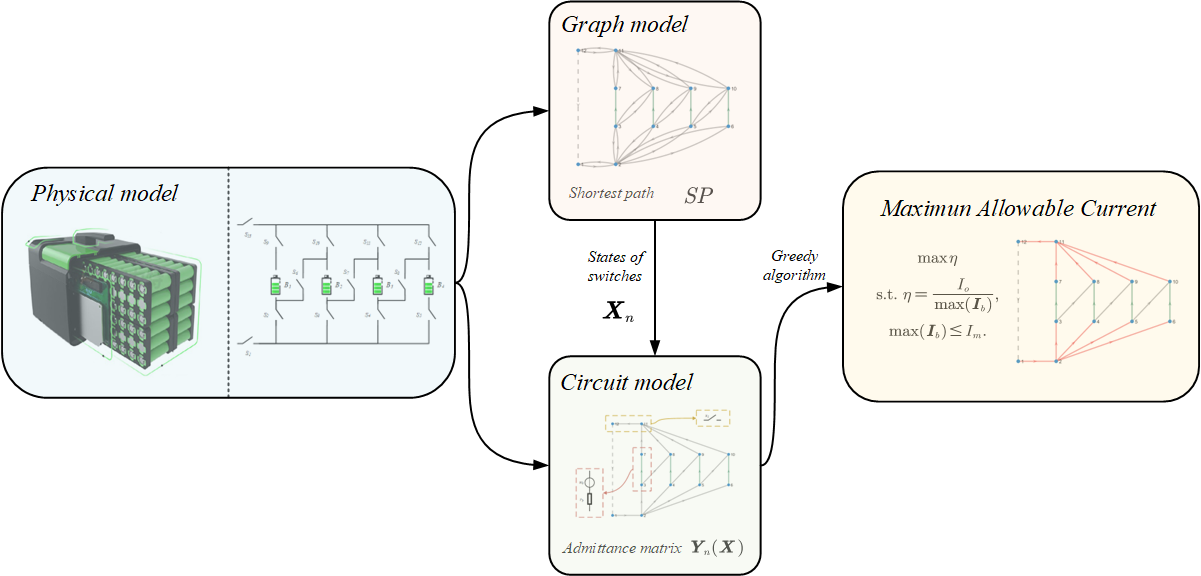
\includegraphics[width=\textwidth]{../attachments/fig1-v2.png}
    \caption{Diagram of our proposed method. It includes a graph model and an equivalent circuit model based on the physical model, and the maximum allowable current is obtained by using a greedy algorithm.}
    \label{fig:1}
\end{figure}


% 【快速评估系统最大电流的作用和意义、文献现状】
% (一些典型结构、控制策略、评估)
% 快速评估系统最大允许电流在设计、分析和控制中起到重要作用。
% 对设计,系统的最大输出电流
% 对控制,应对故障,静态结构破坏
% 但是没有严谨研究最大电流。(直接说没有)
% del: 一些研究使用了过度的简化,不准;(具体文献?):led
% del: 只针对小数量的电池和特定的结构,不普适(具体文献,容易找到):led
Maximum Allowable Current (MAC) is a critical parameter in the design and evaluation of reconfigurable battery systems (RBSs).
MAC determines the maximum current that the RBS can output to external electrical equipment without exceeding a specified current limit for batteries.
This parameter is important for ensuring the safe and reliable operation of RBSs during normal operation and when failed batteries are isolated.
Despite its importance, existing literature on RBSs does not provide a method for calculating MAC, which poses a challenge for the design and evaluation of these systems.


% 【本文的主要内容和结构】
% 我们提出了快速估计RBS的算法,基于贪婪策略。填补了这一空白。
The purpose of this paper is to propose an effective and efficient algorithm based on the greedy search strategy to solve the MAC of RBSs.
A mathematical model of MAC is constructed and the optimal solution is searched in the state space of switches using maximising the number of cells directly connected in parallel as the strategy.

Our main contribution is the development of a mathematical model that describes the problem of calculating the Maximum Allowable Current (MAC) in reconfigurable battery systems (RBSs).
As shown in Figure \ref{fig:1}, the graph model is used to describe the structure of the RBS and determine the shortest paths (SPs) of battery connections to the main circuit with minimal cost;
the circuit model represents the batteries and switches in an actual RBS as equivalent circuit branches that can be processed;
based on a greedy strategy that selects the SPs to determine the switch state $X_s$, we can solve for the optimal MAC.
Our proposed method provides an efficient and effective way to calculate MAC, which can help to improve the design and evaluation of RBSs and ensure their safe and reliable operation in various applications.


% 文章组织:section 2,算法的框架和细节;section 3,案例,讨论和验证;section 4 总结。
This paper is organized as follows.
Section II presents the graph model and circuit model, and the algorithm in detail.
In Section III, we apply the proposed method to solves an example proposed in \cite{kimDESADependableEfficient2012} and further validated its on RBSs of different structures and scales.
Finally, we provides concluding remarks and discuss potential directions for future work.

\section{Method}

\subsection{graph model and circuit model}

A typical RBS circuit is composed of battery cells and switches.
To establish a processable circuit, we transform these components into ideal elements under reasonable assumptions.
The resulting circuit structure is then described in matrix form, and the related equations are provided.

% 【电路,有向图,规定,假设】
% node,连接battery和switch,编号顺序
% edge,battery 或 switch,编号顺序
% 电池等效为恒压ub串内阻rb
% Ro,外电阻
% 关联矩阵
% x,开关状态,01变量
% 【模型,求解方法】
% 假设均一化,矩阵分块
% 在导纳矩阵非奇异的条件下
% 推导出输出电流Io和电池电流Ib

The normal equivalent circuit for a battery consists of a voltage source in series with a resistor, and a capacitor in parallel with another resistor to simulate the polarization in batteries.
Since our main objective is to calculate the stable MAC offered by a given RBS architecture, we only consider the steady-state behavior of the circuit, ignoring transient effects.
Therefore, we model the battery $i$ as a constant voltage source $u_{b,i}$ in series with a resistor $r_{b,i}$.
And we use a binary variable $x_j$ to represent the state of switch $j$, where 0 and 1 indicate open and closed, respectively.
To simplify the calculation, we consider a closed switch as a resistor with a very small resistance value $r_s$, which we treat as zero in the final result.
In the following derivation, we use the product of the conductance $1/r_s$ and the variable $x_j$ to characterize the state of switch $j$.


Before obtaining the incidence matrix representing the structure of the circuit, a directed graph model $G(V,E)$ for the RBS is constructed in such a way that
\begin{enumerate}[(1)]
    \item the vertex set $V={v_1,v_2,\cdots,v_N}$ represents the nodes connecting batteries and/or switches, where $v_1$ and $v_N$ represent the anode and cathode of the RBS respectively;
    \item the directed edge set $E$ represents the output circuit, $N_b$ batteries and $N_s$ switches, corresponding set $E_o$, $E_b$ and $E_s$. The external electrical equipment in the output circuit is treated as one directed edge $v_n \to v_1$. The direction of the edge representing a battery is set to be from the anode to the cathode. For the edges representing switches, their directions are marked from the low node to the the high node. A negative value for the voltage drop or current solved on the edge means that the actual direction is opposite to that initially specified.
\end{enumerate}


Based on the above directed graph which has $N$ nodes and $1+N_b+N_s$ directed edges (1 refers to the output circuit), its incidence matrix $\bm{A}_{N\times (1+N_b+N_s)}$ is defined as
\begin{align}\label{eq:A}
    a_{ij}=
    \begin{cases}
        1,  & \text{edge  $j$ leaves vertex $i$},\\
        -1, & \text{edge $j$ enters vertex $i$},\\
        0,  & \text{otherwise}.
    \end{cases}
\end{align}
Since each column of $\bm{A}$ sums to zero, we delete the last line and use the reduced incidence matrix $\bm{A}_{(N-1)\times(1+N_b+N_s)}$ in the following calculation.
y splitting $E$ into $\{E_o, E_b, E_s\}$, $A$ is rewritten as follows
\begin{equation}
    \bm{A} =
    \begin{bmatrix}
        \bm{A}_o & \bm{A}_b & \bm{A}_s
    \end{bmatrix}.
\end{equation}


$1+N_b+N_s$ edges' currents $\bm{I}_{(1+N_b+N_s)\times 1}$ and voltages $\bm{U}_{(1+N_b+N_s)\times 1}$, and $N-1$ nodes' voltages $\bm{U}_{n, (N-1)\times 1}$ have following relationships from Kirchhoffs law
\begin{align}\label{eq:Kirchhoffs_law}
    \begin{cases}
        \bm{A} \bm{I} = \bm{0}, \\
        \bm{U}        = \bm{A}^\T \bm{U}_n.
    \end{cases}
\end{align}
These directed edges are treated as generalized branches and expressed in matrix form as follows
\begin{equation}\label{eq:generalized_branches}
    \bm{I} = \bm{Y}\bm{X} \bm{U} - \bm{Y}\bm{X} \bm{U}_s +\bm{I}_s,
\end{equation}
where $\bm{I}$ and $\bm{U}$ are the column vectors about $1+N_b+N_s$ edges' current and voltage, respectively;
$\bm{U}_s$ and $\bm{I}_s$ denote the source voltage and source current of the generalized branches, respectively;
$\bm{Y}$ is the admittance matrix of the circuit, and $\bm{X}$ is the state matrix defined as
\begin{equation}\label{eq:X}
    \bm{X} = diag(
    1,
    \underbrace{1, \cdots, 1}_{N_b~\text{of}~1},
    \underbrace{1, 0 \cdots, 1}_{N_s~\text{of}~0/1}
    )
    =\begin{bmatrix}
        \bm{I} &\\
        & \bm{X}_s
    \end{bmatrix}.
\end{equation}


In addition to the equivalent circuit assumptions, we also assume that all batteries have the same internal resistance value $r_b$ and supply the same electric potential $u_s$ to simplify the model.
Then the output current $I_o$ and each battery's current $\bm{I}_b$ can be given by solving the simultaneous Equations \ref{eq:Kirchhoffs_law} and \ref{eq:generalized_branches} eventually.
Let
\begin{equation}\label{eq:Yn}
    \bm{Y}_n (\bm{X}) = \frac{1}{R_o} \bm{A}_o\bm{A}_o^\T + \frac{1}{r_b} \bm{A}_b\bm{A}_b^\T + \frac{1}{r_s}\bm{A}_s\bm{X}_s\bm{A}_s^\T,
\end{equation}
% \begin{equation}\label{eq:Yn}
%     \bm{Y}_n (\bm{X}_s) = \frac{1}{R_o} \bm{A}_o\bm{A}_o^\T + \bm{A}_b \bm{Y}_b \bm{A}_b^\T + \bm{A}_s \bm{Y}_s \bm{X}_s \bm{A}_s^\T
% \end{equation}
where $R_o$ is the equivalent resistance of the external circuit.
Then, if $\bm{Y}_n$ is an invertible matrix,
\begin{align}
    I_o(\bm{X})      & = \frac{u_b}{R_o r_b} \bm{A}_o^\T \bm{Y}_n^{-1}(\bm{X}) \bm{A}_b \bm{I}_{N_b\times 1};\label{eq:I_o}\\
    \bm{I}_b(\bm{X}) & = \frac{u_b}{r_b^2}[\bm{A}_b^\T \bm{Y}_n^{-1}(\bm{X}) \bm{A}_b\bm{I}_{N_b \times 1}  -r_b \bm{I}_{N_b \times 1}],\label{eq:I_b}
\end{align}
% \begin{align}
%     I_o(\bm{X}_s)      & = \frac{1}{R_o}\bm{A}_o^\T\bm{Y}_n^{-1}(\bm{X}_s)\bm{A}_b\bm{Y}_b\bm{U}_b;\label{eq:I_o}\\
%     \bm{I}_b(\bm{X}_s) & = \bm{Y}_b\bm{A}_b^\T\bm{Y}_n^{-1}(\bm{X}_s)\bm{A}_b\bm{Y}_b\bm{U}_b-\bm{Y}_b\bm{U}_b,\label{eq:I_b}
% \end{align}
where $\bm{I}_{N_b\times 1}$ is a column vector with all terms being one.


% 用外电流Ib比所有电池中最大电流max(Ib)之比,表征电路的最大许用输出。是电路结构本身的性质,与电池无关。电路的线性保证了。
% 目标问题转化为【数学形式】
% Max rate
% s.t.
We use the ratio of $I_o$ and $\max (\bm{I}_b)$ to characterize the allowable current for a given RBS architecture, denoted as $\eta$.
The $\eta$ reflects the ability of the RBS architecture itself to deliver current, regardliess of the battery cells used by the RBS.
Due to the linearity of the above circuit model, the output current will vary by the same multiple if the allowable current of all batteries varies by a certain multiple.
Our problem in RBS can be formulated as
\begin{align}
    & \max \eta \label{eq:max_eta}\\
    \mathrm{s.t.}\,\, & \eta = \frac{I_o}{\max (\bm{I}_b)}, \\
    & \max (\bm{I}_b) \leq I_m,
\end{align}
where $I_m$ is the maximum allowable current of the battery; $I_o$ and $\bm{I}_b$ can be calculated by Equations \ref{eq:I_o} and \ref{eq:I_b}.
The presence of the inverse matrix $\bm{Y}_n^{-1}$ prevents us from solving \ref{eq:max_eta} directly, especially when a large number of battery cells and switches are present in the system.
We therefore propose a greedy algorithm to solve this model.


\subsection{greedy solution}
% 使用贪心算法策略求解
% 【贪心策略】
% 电池i的最短路径,短指的是路径上电池数量最少
% 贪心策略,当系统中越多的电池被以最短路径联入电路,外电路电流越大。
% 短路,检查
% 组合,逐一
First, we define the battery $i$'s shortest path ($SP_i$).
When the battery $i$ is connected to the anode $v_1$ and the cathode $v_N$ of the RBS by the path $p$ in the graph model, the distance $\omega$ of $p$ is defined by the following equation:
\begin{equation}\label{eq:weight}
    \omega(p) = N_s \cdot n_b (p) + n_s (p),
\end{equation}
where $N_s$ is the total number of switches in the system; $n_b(p)$ and $n_s(p)$ are number of batteries and switches in the path $p$ respectively.
$SP_i$ is defined as the path with the minimum $\omega$ for battery $i$.
According to the definition, $SP_i$ gives the simplest strategy by which the control of battery $i$ is achieved with a minimum of switches while minimising the influence of other batteries.
From the perspective of series/parallel, the more batteries are connected into circuit via their $SP$s, the more batteries are connected in parallel.
Since batteries can provide more total output current when connected in parallel than in series, we greedily allow as many cells as possible to be connected into to the overall circuit via their $SP$s to obtain the MAC.
The dichotomy method is also performed to faster find the right number of $SP$s.



% 【总体流程(二分查找)】
% 对于给定结构和最大许用电流通过如下步骤得到:
% (伪代码开始)
% 通过图查找,深度优先,对每个电池找最短路径
% 以二分策略选择考察电池数量N_{select}
% 通过组合,形成C^{N_select}_{N_total}种方式,对于每种方式
%   仅将选中的电池最短路径上的开关状态设置为1
%   求解电流,公式
%   检查各电池电流,是否短路或超过电池的最大许用电流(否,break)
%   给出外电路电流和所有电池电流的最大值,计算比率
% (伪代码结束)
% 电池电流Ib不超过ub/rb,未短路,合法(电池电流Ib受外电路Ro影响,考虑设一个固定值Ibmax,表示电池最大许用电流)
The pseudo-code of the algorithm is as follows:
\begin{algorithm}
    \caption{Get the max available currents of a certain RBS}\label{alg:eta_RBS}
    \KwData{Directed graph model $G(V,E)$ of the RBS}
    \KwResult{$\max \eta$}
    \For{$i \in E_b$}{
        $P_i \leftarrow \{path| \text{starts at $v_1$ and ends at $v_n$} \}$\;
        $SP_i \leftarrow p_i \text{ which has the minimum}~\omega(p_i)~\text{among all}~p_i \in P_i. $
    }
    get $\bm{A}$ by Equation \ref{eq:A}\;
    \While{not yet determine $\max \eta$ }
    {
        $N_{sel} \leftarrow \text{number of selected $SP$s calculated by dichotomy}$\;
        $C_b    \leftarrow \text{set of all combinations of $N_{sel} $~batteries from $N_b$}$\;
        \For{$c_b \in C_b$}{
            % $P_{selected} \leftarrow \bigcup_{i\in c_b}SP_i$\;
            $\bm{x}_s \leftarrow \text{list of all switches' state: $x_s[j]=1$ if $ j \in \bigcup_{i\in c_b}SP_i $ else 0}$\;
            $\bm{X} \leftarrow diag[1,1,\cdots,1,\bm{x}_s] $\;
            get $\bm{Y}_n$ by Equation \ref{eq:Yn}\;
            \eIf{$\bm{Y}_n$ is invertible}{
            }{construct an effective solution}
            get $I_o$ by Equation \ref{eq:I_o}\;
            get $\bm{I}_b$ by Equation \ref{eq:I_b}\;
            \eIf{$\max(\bm{I}_b)\leq I_m$}{
                $\eta \leftarrow I_o/\max(\bm{I}_b)$\;
            }{break}
        }
    }
\end{algorithm}

\section{Examples and discussions}
% 经典结构  visairoReconfigurableBatteryPack2008 验证我们方法的有效性,这个结构的设计目的和应用,我们的验证基于不同规模
% 建模:物理结构,图模型,电路模型
% 求解及讨论:模型的正确性,不同规模的效率


% 1. 以f4结构为例,example
% 描述试验过程,包括物理模型(结构)、图模型(有向图、SP)、电路模型(关联矩阵和状态向量)
% 描述试验结果,根据求解算法,当SPs取xxx时,电路输出电流达到MAC(图,红色表示开关闭合),各电池电流、输出电流的符号运算结果
% 讨论结果,关联矩阵A的可逆性讨论;影响输出电流的因素,对MAC定义的讨论,对“许用”的说明;
% 2. 为进一步说明模型和算法的有效性,我们对不同结构、不同电池规模进行求解
% a). 在e4、f4、e2f2结构上验证算法有效性
% b). 在f2、f4、f6、f12 上验证有效性
% (图)物理模型、求解后模型、求解结果:红色表示开关闭合
% (图)说明电池数量增加的示意图
% (表)结构、求解结果(Io,Ibmax,MAC)
% (表)电池数量、求解结果(Io,Ibmax,MAC)
% 准确性:算法MAC求解结果与电路定律符合
% 正确性:模型将电池的物理模型等效为恒压源和电阻,外电路等效为电阻,验证该假设的合理性——分析ub、rb等对结果的影响
% 3. 该方法的优点和未来改进方向:
% a) 可以获得电路的所有信息,用于其他可重构电路指标的计算,如输出电压等
% b) 可对电池等效模型进行修改,如引入电容,分析暂态


In this section, we evaluate the algorithm and models for MAC mentioned earlier, based on some previously reported structures.
Firstly, we provide a specific example for the algorithm and models proposed in Section II using the structure proposed by Visairo and discuss the model and computation process.
Next, we further verify the applicability of our method on RBSs with different structures and sizes.
Finally, we highlight the advantages of our method and suggest directions for future improvements.


\subsection{An specific example}

\begin{figure}[htbp]
    \centering
    \begin{subfigure}[b]{0.45\textwidth}
        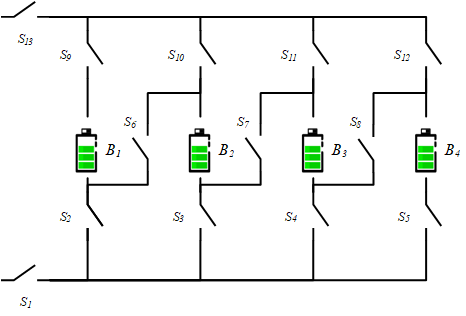
\includegraphics[width=\textwidth]{../attachments/f4-phy.png}
        \caption{}
        \label{fig:f4-phy}
    \end{subfigure}
    \hspace{0.05\textwidth}
    \begin{subfigure}[b]{0.45\textwidth}
        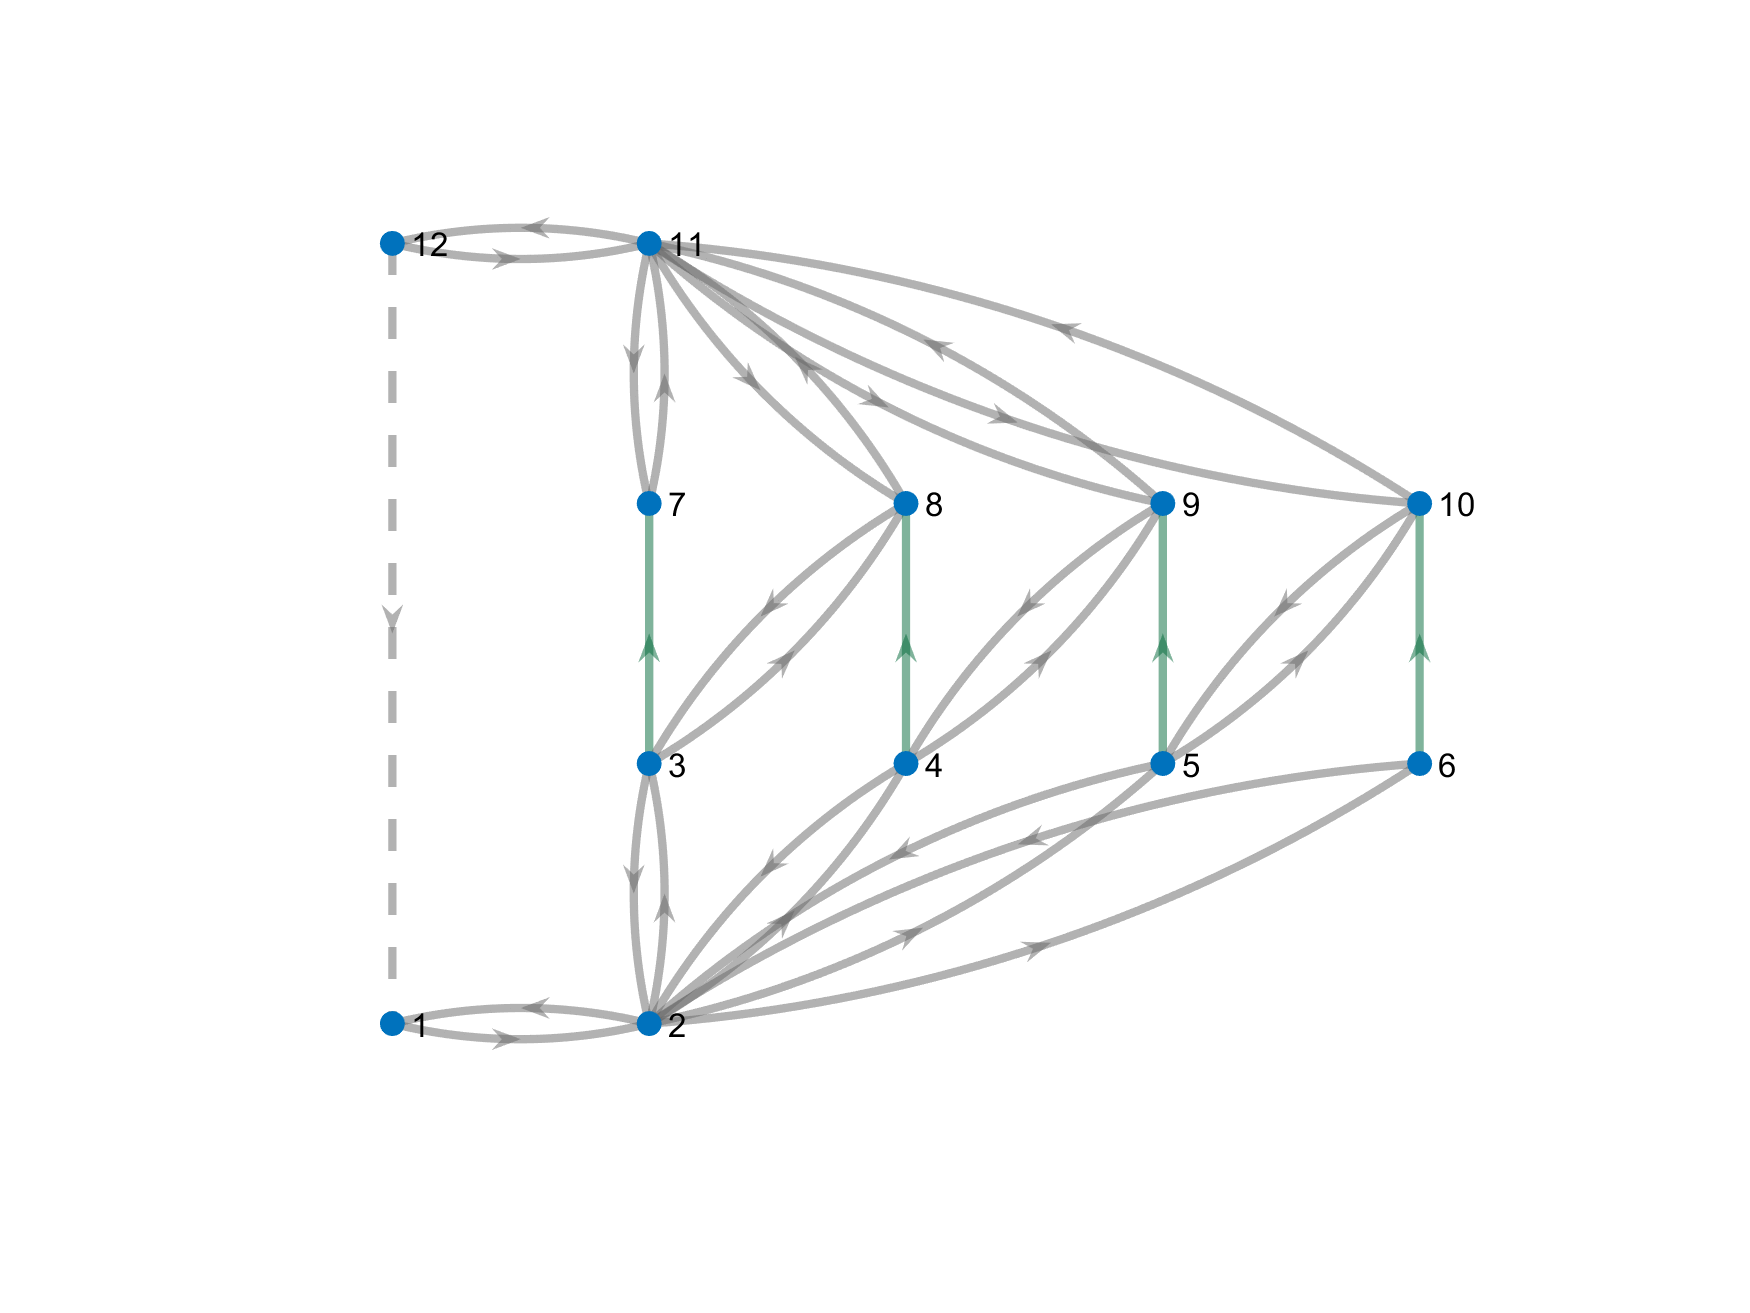
\includegraphics[width=\textwidth]{../attachments/f4-gra.png}
        \caption{}
        \label{fig:f4-gra}
    \end{subfigure}
    \\
    \begin{subfigure}[b]{0.45\textwidth}
        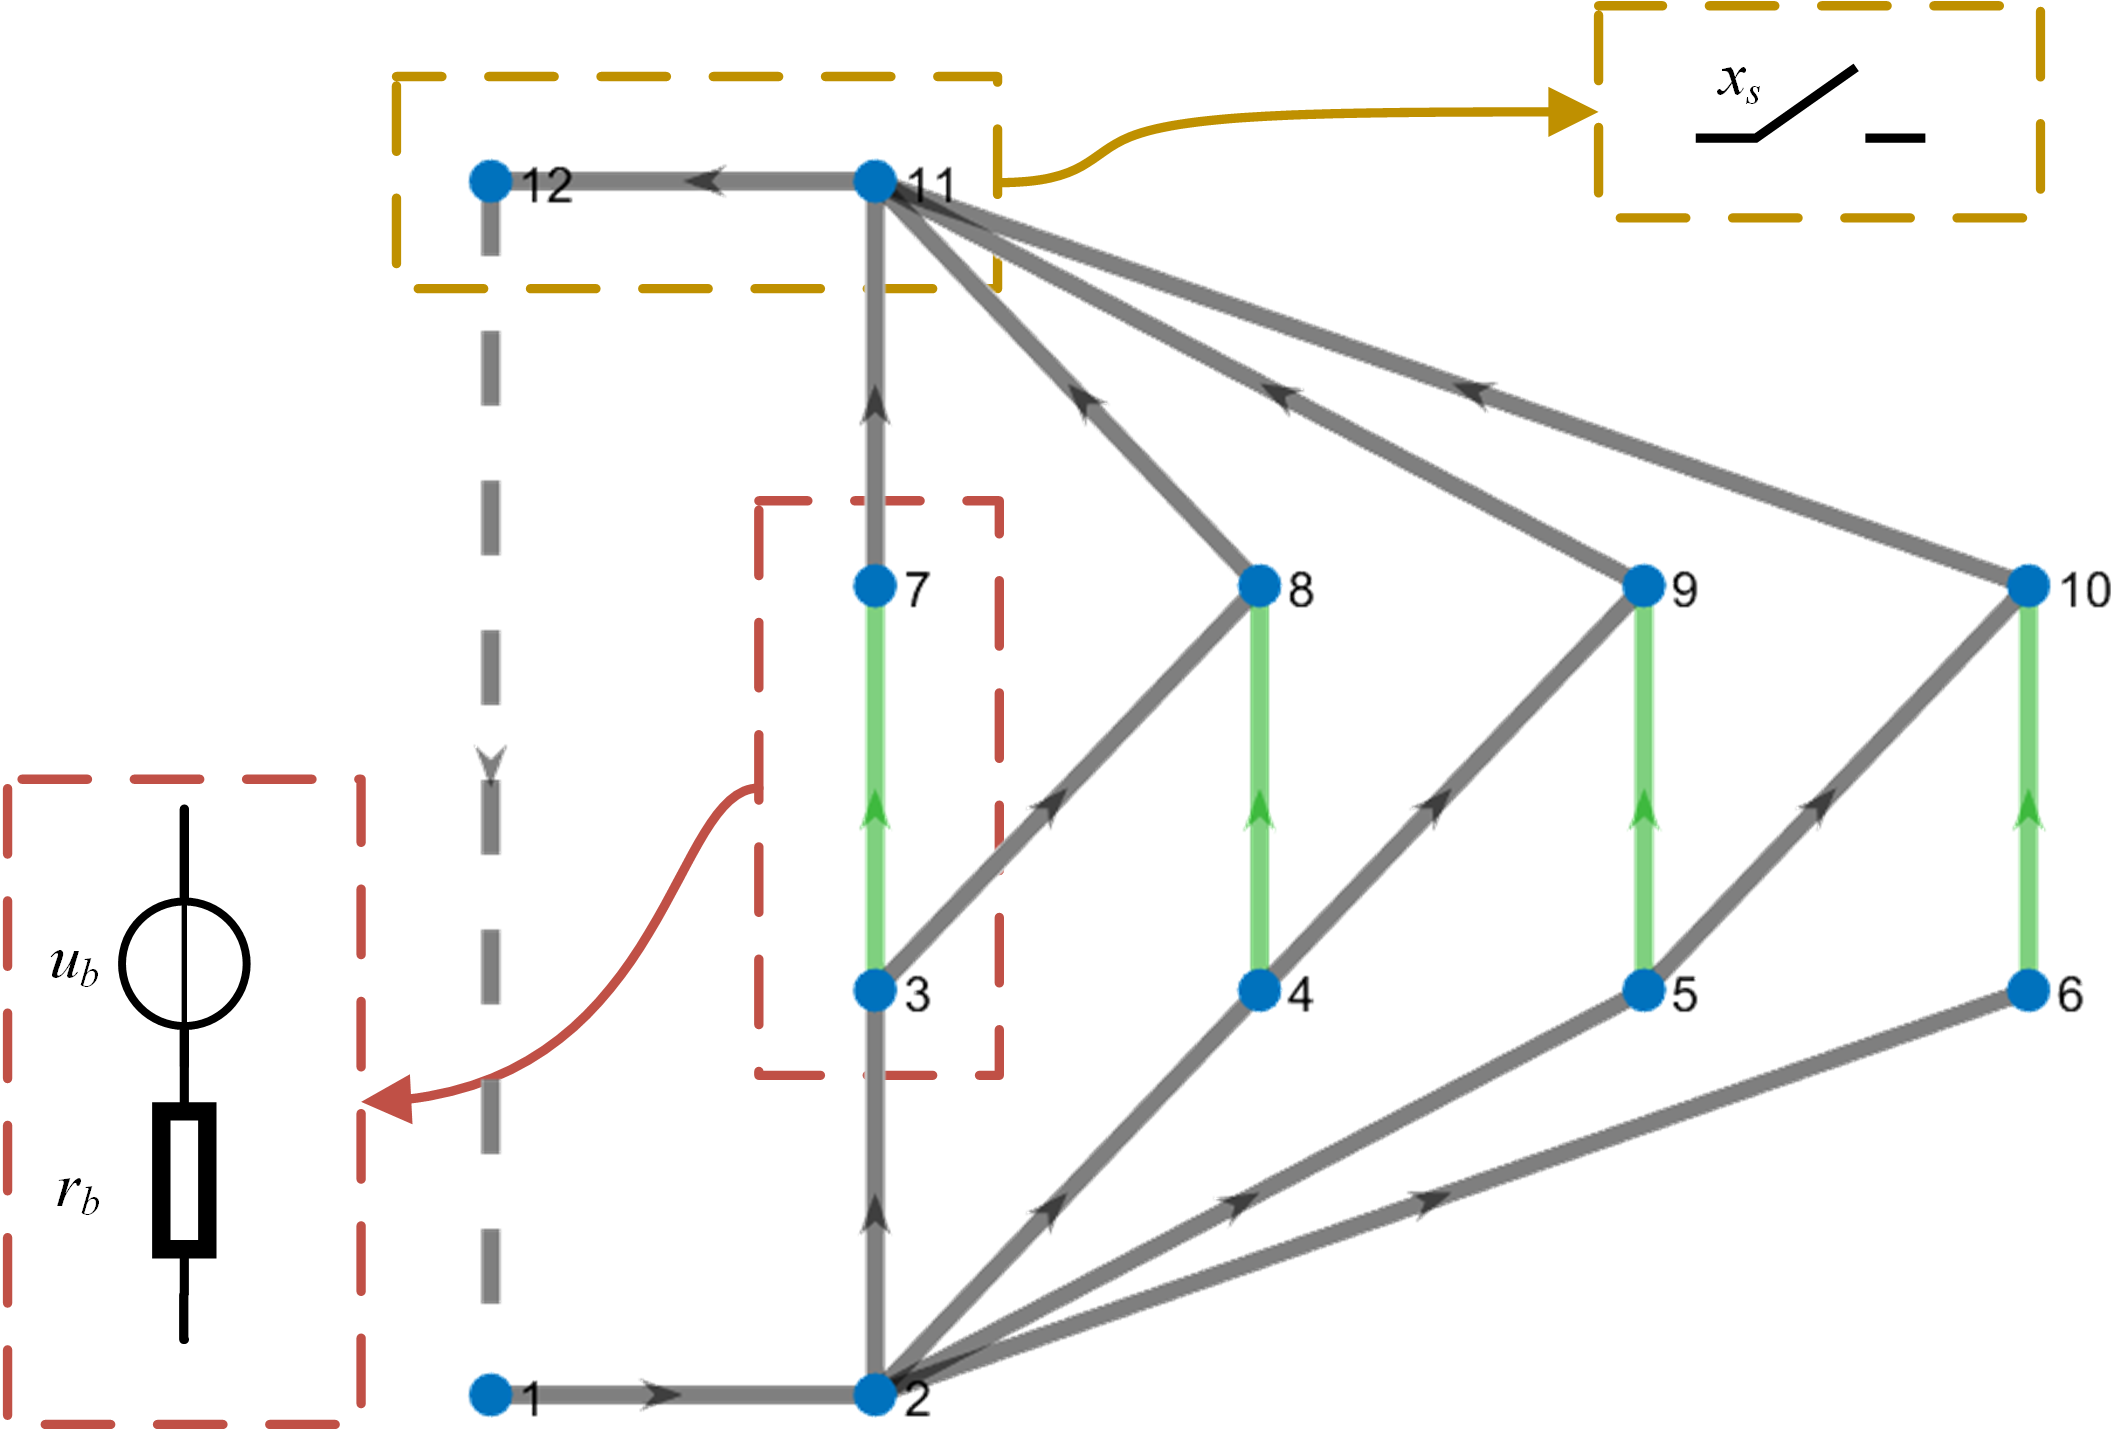
\includegraphics[width=\textwidth]{../attachments/f-dege-4-modify.png}
        \caption{}
        \label{fig:f4-circ}
    \end{subfigure}
    \hspace{0.05\textwidth}
    \begin{subfigure}[b]{0.45\textwidth}
        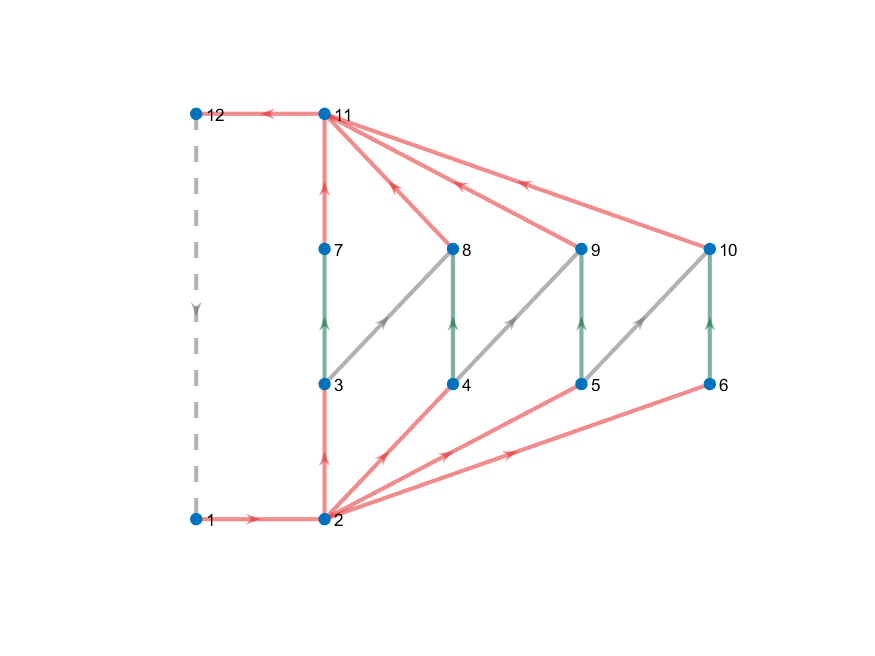
\includegraphics[width=\textwidth]{../attachments/f-dege-mac-4.png}
        \caption{}
        \label{fig:f4-mac}
    \end{subfigure}
    \caption{ RBS structure proposed by Visairo\cite{visairoReconfigurableBatteryPack2008} with 4 batteries. (a) Physical model, (b) graph model, (c) equivalent circuit model, and (d) results obtained by using the proposed method. The red highlighted lines indicate the open/close states of switches.}
    \label{fig:f4-all}
\end{figure}


The reconfigurable architecture proposed by Visairo et al.\cite{visairoReconfigurableBatteryPack2008} is shown in Figure \ref{fig:f4-phy}.
In this architecture, each cell is controlled by about 3 switches on average.
Excepted for two switches ($S_1$ and $S_{13}$ in Figure \ref{fig:f4-phy}) controlling the total circuit, the vertical switches (e.g. $S_2$ and $S_9$ in Figure \ref{fig:f4-phy}) allow the batteries to be directly connected to the main circuit, and the switches($S_6$ for example) in the diagonal direction can realize connecting the batteries in series.
Thus, it can dynamically change the output voltage and current as needed.
The architecture in Figure \ref{fig:f4-phy} only has 4 batteries, but in practice it can add new branches containing batteries and switches to deal with large-scale batteries\cite{kimDependableEfficientScalable2010}.


The graph in Figure \ref{fig:f4-gra} represents a graphical model based on the physical model(Figure \ref{fig:f4-phy}).
The model is presented in the form of a directed graph, capturing the connection relationship between the battery and switch in the circuit.
Vertex 1 and 12 represent the ancode and cathode of the RBS, respectively;
the remaining vertices represent the connection nodes between the batteries and switches.
Battery 1, 2, 3, and 4 are represented by green directed edges in the graph, while switches are represented by gray directed edges with opposite directions.
The external electrical appliance is considered as a directed edge from node 12 to node 1.
In the graph model, the directionality of the edges is strictly specified to ensure that there is no reverse flow of current in the battery and external electrical appliance, which could damage the appliance.


According to Equation \ref{eq:weight}, the weight of the edge corresponding to the battery is the total number of switches, which is 13;
the weight of the edge corresponding to the switch is 1.
By setting the weight in this way, on the one hand, it avoids the simultaneous occurrence of multiple batteries in a single SP, weakening the influence between different batteries;
on the other hand, it minimizes the number of switches on the path, which means that only a few switches (i.e., the switches on the SP) need to be closed to connect the battery to the main circuit.
By using the depth-first search algorithm, the SP of battery 1 can be calculated as the node list $[1, 2, 3, 7, 11, 12]$, and the SPs of the other batteries are shown in Figure \ref{fig:f4-gra}.
The SPs provide a basis for selecting variables when solving the MAC through the circuit model in the future.


The equivalent circuit model, as shows in Figure \ref{fig:f4-circ}, can be obtained based on the assumptions in Section II.
In this model, the batteries and switches are treated as branches, where the battery is regarded as a branch consisting of a voltage source $u_b$ in series with a resistor $r_b$, and the switch is regarded as a branch controlled by a state variable $x_s$ to short or open the circuit.
Difference from the directed graph model, only one directed edge is used to represent the branch in the circuit, regardless of whether it represents a battery or a switch.
The direction of the edge is defined as pointing from the node with the smaller number to the  larger .
The direction of the edge is only a preset direction used to calculate the current and voltage.
When the computed current or voltage value is negative, it indicates that the direction of the battery or potential difference is opposite to the preset direction.
Based on the node-edge relationship in Figure \ref{fig:f4-circ}, the incidence matrix $\bm{A}$: can be obtained according to Equation \ref{eq:A}:
% {\setlength{\arraycolsep}{4pt}
% \begin{equation}
% \begin{array}{cc}
%     &  \begin{array}{c c ccc cccccccccc} & e_o &e_{b1}  &e_{b2} & e_{b3} & e_{s1} & e_{s2} & e_{s3} & e_{s4} & e_{s5} & e_{s6} & e_{s7} & e_{s8} & e_{s9} & e_{s10} \end{array}\\
%         \begin{array}{c} v_1\\v_2\\v_3\\v_4\\v_5\\v_6\\v_7\\v_8\\v_9\end{array} & \left[
%     \begin{array}{c|ccc|cccccccccc}
%         -1  &0 &0 &0   &1 &0 &0 &0 &0 &0 &0 &0 &0 &0\\
%         0   &0 &0 &0   &-1&1 &1 &1 &0 &0 &0 &0 &0 &0\\
%         0   &1 &0 &0   &0 &-1&0 &0 &1 &0 &0 &0 &0 &0\\
%         0   &0 &1 &0   &0 &0 &-1&0 &0 &1 &0 &0 &0 &0\\
%         0   &0 &0 &1   &0 &0 &0 &-1&0 &0 &0 &0 &0 &0\\
%         0   &-1&0 &0   &0 &0 &0 &0 &0 &0 &1 &0 &0 &0\\
%         0   &0 &-1&0   &0 &0 &0 &0 &-1&0 &0 &1 &0 &0\\
%         0   &0 &0 &-1  &0 &0 &0 &0 &0 &-1&0 &0 &1 &0\\
%         0   &0 &0 &0   &0 &0 &0 &0 &0 &0 &-1&-1&-1&1\\
%     \end{array} \right]
% \end{array},
% \end{equation}
% }
{\setlength{\arraycolsep}{2pt}
\begin{equation}
    \begin{array}{cc}
        &  \begin{array}{c c cccc ccccccccccccc} & e_o &e_{b1}  &e_{b2} & e_{b3} & e_{b4} & e_{s1} & e_{s2} & e_{s3} & e_{s4} & e_{s5} & e_{s6} & e_{s7} & e_{s8} & e_{s9} & e_{s10} & e_{s11} & e_{s12} & e_{s13} \end{array}\\
            \begin{array}{c} v_1\\v_2\\v_3\\v_4\\v_5\\v_6\\v_7\\v_8\\v_9\\v_{10}\\v_{11}\\v_{12}\end{array} & \left[
                    \begin{array}{c|cccc|ccccccccccccc}
                        -1  &  0  &  0  &  0  &  0  &  1  &  0  &  0  &  0  &  0  &  0  &  0  &  0  &  0  &  0  &  0  &  0  &  0\\
                        0  &  0  &  0  &  0  &  0  & -1  &  1  &  1  &  1  &  1  &  0  &  0  &  0  &  0  &  0  &  0  &  0  &  0\\
                        0  &  1  &  0  &  0  &  0  &  0  & -1  &  0  &  0  &  0  &  1  &  0  &  0  &  0  &  0  &  0  &  0  &  0\\
                        0  &  0  &  1  &  0  &  0  &  0  &  0  & -1  &  0  &  0  &  0  &  1  &  0  &  0  &  0  &  0  &  0  &  0\\
                        0  &  0  &  0  &  1  &  0  &  0  &  0  &  0  & -1  &  0  &  0  &  0  &  1  &  0  &  0  &  0  &  0  &  0\\
                        0  &  0  &  0  &  0  &  1  &  0  &  0  &  0  &  0  & -1  &  0  &  0  &  0  &  0  &  0  &  0  &  0  &  0\\
                        0  & -1  &  0  &  0  &  0  &  0  &  0  &  0  &  0  &  0  &  0  &  0  &  0  &  1  &  0  &  0  &  0  &  0\\
                        0  &  0  & -1  &  0  &  0  &  0  &  0  &  0  &  0  &  0  & -1  &  0  &  0  &  0  &  1  &  0  &  0  &  0\\
                        0  &  0  &  0  & -1  &  0  &  0  &  0  &  0  &  0  &  0  &  0  & -1  &  0  &  0  &  0  &  1  &  0  &  0\\
                        0  &  0  &  0  &  0  & -1  &  0  &  0  &  0  &  0  &  0  &  0  &  0  & -1  &  0  &  0  &  0  &  1  &  0\\
                        0  &  0  &  0  &  0  &  0  &  0  &  0  &  0  &  0  &  0  &  0  &  0  &  0  & -1  & -1  & -1  & -1  &  1\\
                    \end{array} \right]
    \end{array},
\end{equation}
}
where the rows correspond to vertexes in the graph model, and the first column, second to fourth columns, and last ten columns correspond to external electrical equipment, 4 batteries, and 13 switches, respectively.
According to the above classification of the columns, the matrix $\bm{A}$ can be divided into $\bm{A}_o$, $\bm{A}_b$, and $\bm{A}_s$.


The state matrix $\bm{X}$ is determined by the switches' state, that is, the specific configuration of the RBS.
For example, when switch
% $S_1$, $S_2$, $S_3$, $S_4$ , $S_7$, $S_8$, $S_9$ and $S_{10}$  % for f3
$S_1$, $S_2$, $S_3$, $S_4$, $S_5$, $S_9$, $S_{10}$, $S_{11}$, $S_{12}$ and $S_{13}$
are closed, and switch $S_6$, $S_7$ and $S_8$ are open, that is , battery $B_1$, $B_2$, $B_3$ and $_4$ are connected in parallel to supply power to the external circuit, the state matrix $\bm{X}$ is given by
\begin{equation}
    %     \bm{X} = diag(
    %         1,
    %         \underbrace{1,1,1}_{\text{batteries}},
    %         \underbrace{1,1,1,1,0,0,1,1,1,1}_{\text{switches}}
    %     ).
    \bm{X} = diag(
    1,
    \underbrace{1,1,1,1}_{\text{batteries}},
    \underbrace{1,1,1,1,1,0,0,0,1,1,1,1,1}_{\text{switches}}
    ).
\end{equation}


When using Algorithm 1 to solve the MAC, we may encounter the situation where the matrix $\bm{Y}_n$ is not full rank, and we cannot directly obtain its inverse matrix.
This is because some switches are open, causing some branches with voltage sources to be independent of the main circuit and form new circuits.
These circuits have infinite possible values for potential difference between them, since they are not connected to each other.
In other words, there are theoretically infinite solutions for potential.
However, all of these solutions will satisfy the voltage and current laws required by the equation.
On the one hand, for the main circuit, since the model specifies node 12 as the reference point for potential at the beginning (i.e., the associated matrix $\bm{A}$ is reduced by one row corresponding to node 12), the submatrix of $\bm{Y}_n$ formed by the edges on the main circuit path must be full rank, so there is no problem as described above.
On the other hand, since the new circuit is independent of the main circuit, it will not affect the output currents of the main circuit and the battery currents.
Therefore, any solution can be used for subsequent calculations.
Here, we can choose the solution where the potential at the node with the smallest number in the independent branch is 0.

% MAC of RBS_f(4): 4.00
% Io_ideal: (4*ub)/(4*Ro + rb)
% Ib_ideal(1): ub/(4*Ro + rb)
% Ib_ideal(2): ub/(4*Ro + rb)
% Ib_ideal(3): ub/(4*Ro + rb)
% Ib_ideal(4): ub/(4*Ro + rb)
% those switches are close: 1 2 3 4 5 9 10 11 12 13
The final calculation result of $\eta$ for the structure in Figure \ref{fig:f4-phy} is 4.
The corresponding currents of output and each battery are shown in Table \ref{tab:1}.
The red edges in Figure \ref{fig:f4-mac} represent the closed switches.
\begin{table}[h]
    \caption{Detailed results of the proposed method for the RBS structure proposed by Visairo\cite{visairoReconfigurableBatteryPack2008} with 4 batteries, including the output current, current of each battery, and $\eta$.}
    \label{tab:1}
    \begin{tabular}{ccc}
        \hline
        output current $I_o$       & battery current $\bm{I}_b$       & $\eta$        \\
        \hline\\
        $\displaystyle\frac{4u_b}{4R_o + r_b}$ &  $\displaystyle\left[\frac{u_b}{4R_o + r_b},\frac{u_b}{4R_o + r_b},\frac{u_b}{4R_o + r_b},\frac{u_b}{4R_o + r_b}\right]$   & $4.00$ \\
        \\
        \hline
    \end{tabular}
\end{table}
For this structure, when all batteries are connected to the main circuit through the switches in the vertical direction in Figure \ref{fig:f4-phy} and the batteries are connected in parallel, the output current is maximum, which is the sum of the currents of the four batteries.
The MAC of this structure is correctly estimated by our greedy algorithm.
From the specific results of the output current $I_o$ and battery currents $\bm{I}_b$, both are related to the battery voltage $u_b$, internal resistance $r_b$, and external circuit resistance $R_o$.
This means that even for the same structure, the output current will change when the external circuit  or the battery specifications  change.
By dividing the output current by the sum of the battery currents, we obtain $\eta$, in which the effects of these variables cancel out.
Thanks to the linearity of the studied structure, when the battery specifications change, the output current also changes proportionally, such as doubling the battery voltage would also double the output current.
This variable can reflect the characteristics of the structure itself, regardless of the batteries used.
Therefore, using $\eta$ as the metric for the MAC is better than using the output current directly.

\subsection{Difference structures and sizes}

To further demonstrate the effectiveness of the model and algorithm, we solve for different structures and RBSs of different sizes.


Figure \ref{fig:d-structure} illustrates three architectures, each consisting of four batteries with different interconnections.
Architecture \ref{fig:d-structure-f4}, previously described in the subsection, was proposed by Visairo\cite{visairoReconfigurableBatteryPack2008}.
Architecture \ref{fig:d-structure-e4}, proposed by Lawson \cite{lawsonSoftwareConfigurableBattery2012}, allows for the disconnection of any battery to isolate a faulty one or to provide redundancy, and requires significantly fewer switches than \ref{fig:d-structure-e4}.
Architecture \ref{fig:d-structure-e2f2} is a novel structure obtained by combining the features of both \ref{fig:d-structure-f4} and \ref{fig:d-structure-e4}.
The final solution obtained by the greedy algorithm is shown in Figure \ref{fig:d-structure} and summarized in Table \ref{tab:d-structure}.
\begin{figure}[htbp]
    \centering
    \begin{subfigure}[b]{0.3\textwidth}
        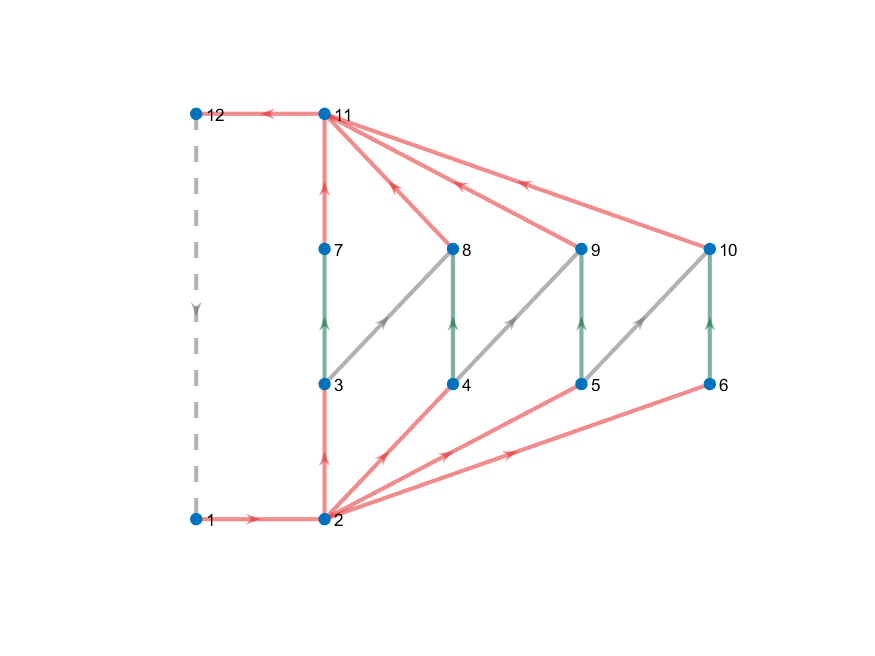
\includegraphics[width=\textwidth]{../attachments/f-dege-mac-4.png}
        \caption{}
        \label{fig:d-structure-f4}
    \end{subfigure}
    \hspace{0.05\textwidth}
    \begin{subfigure}[b]{0.3\textwidth}
        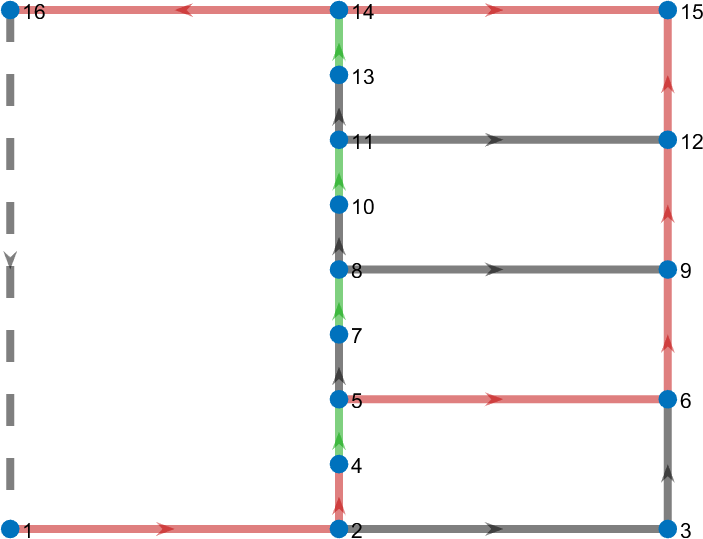
\includegraphics[width=\textwidth]{../attachments/e-dege-mac-4.png}
        \caption{}
        \label{fig:d-structure-e4}
    \end{subfigure}
    \hspace{0.05\textwidth}
    \begin{subfigure}[b]{0.45\textwidth}
        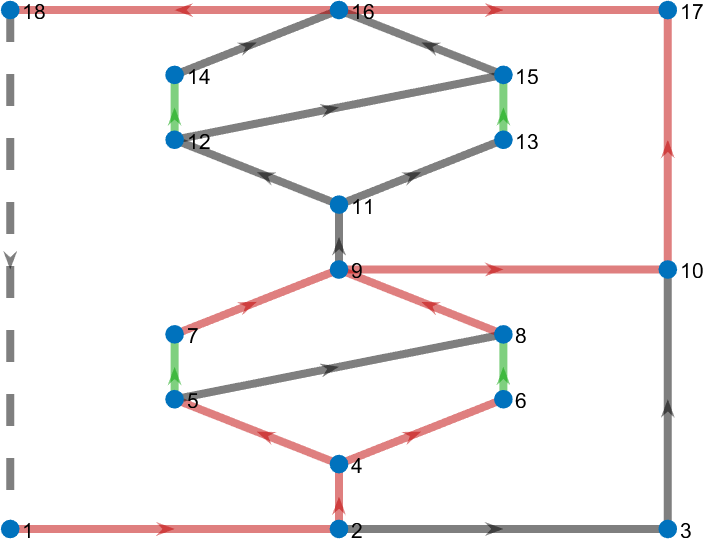
\includegraphics[width=\textwidth]{../attachments/e2f2-dege-mac.png}
        \caption{}
        \label{fig:d-structure-e2f2}
    \end{subfigure}
    \caption{Results obstained by our method on (a) structure proposed by Visairo\cite{visairoReconfigurableBatteryPack2008}, (b) structure proposed by Lawson\cite{lawsonSoftwareConfigurableBattery2012}, and (c) structure combining Visairo's and Lawson's structure. The red highlighted lines indicate the open/close states of switches.}
    \label{fig:d-structure}
\end{figure}


\begin{table}[h]
    \centering
    \caption{detailed results of the proposed method for the rbs structure with 4 batteries (a) proposed by visairo\cite{visairoReconfigurableBatteryPack2008}, (b) proposed by lawson\cite{lawsonSoftwareConfigurableBattery2012} and (c) combining both  , including the output current, current of each battery, and $\eta$.}
    \label{tab:d-structure}
    \begin{tabular}{cccc}
        \hline
        structure &  output current $I_o$       & battery current $\bm{I}_b$       & $\eta$        \\
        \hline\\
        Visairo\cite{visairoReconfigurableBatteryPack2008} &  $\displaystyle\frac{4u_b}{4R_o + r_b}$ &  $\displaystyle\left[\frac{u_b}{4R_o + r_b},\frac{u_b}{4R_o + r_b},\frac{u_b}{4R_o + r_b},\frac{u_b}{4R_o + r_b}\right]$   & $2.00$ \\
        \\
        Lawson\cite{lawsonSoftwareConfigurableBattery2012} &  $\displaystyle\frac{u_b}{R_o + r_b}$ &  $\displaystyle\left[\frac{u_b}{R_o + r_b},0,0,0\right]$   & $4.00$ \\
        \\
        combining both &  $\displaystyle\frac{2u_b}{2R_o + r_b}$ &  $\displaystyle\left[\frac{u_b}{2R_o + r_b},\frac{u_b}{2R_o + r_b},0,0\right]$   & $6.00$ \\
        \\
        \hline
    \end{tabular}
\end{table}

Figure \ref{fig:d-size} presents the structures proposed by Visairo \cite{visairoReconfigurableBatteryPack2008} with varying numbers of batteries.
We applied our method to solve structures with 2, 4, and 6 batteries, and the results are shown in Figure \ref{fig:d-size} and summarized in Table \ref{tab:d-size}.

\begin{figure}[htbp]
    \centering
    \begin{subfigure}[b]{0.3\textwidth}
        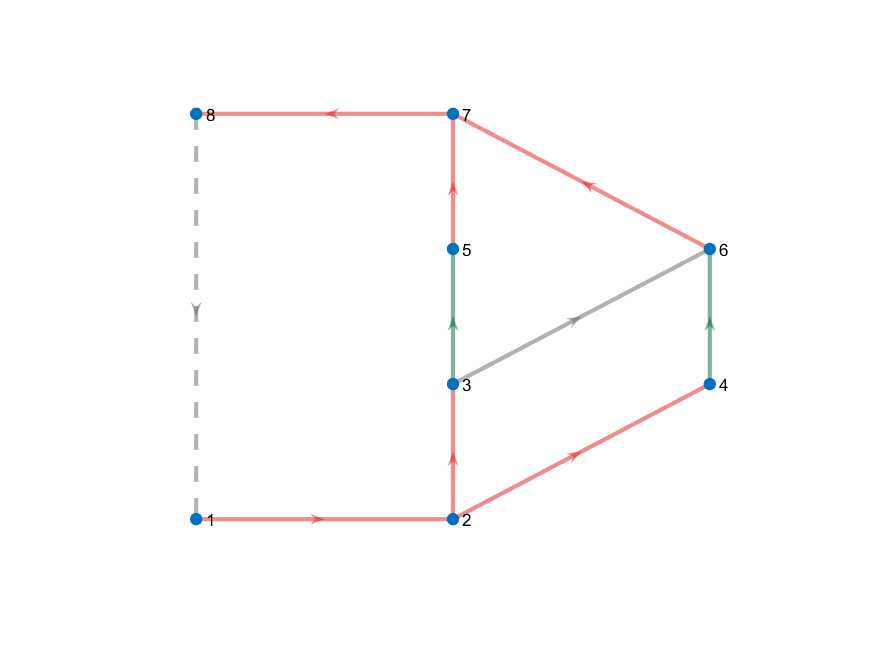
\includegraphics[width=\textwidth]{../attachments/f-dege-mac-2.png}
        \caption{}
        \label{fig:d-size-2}
    \end{subfigure}
    \hspace{0.05\textwidth}
    \begin{subfigure}[b]{0.3\textwidth}
        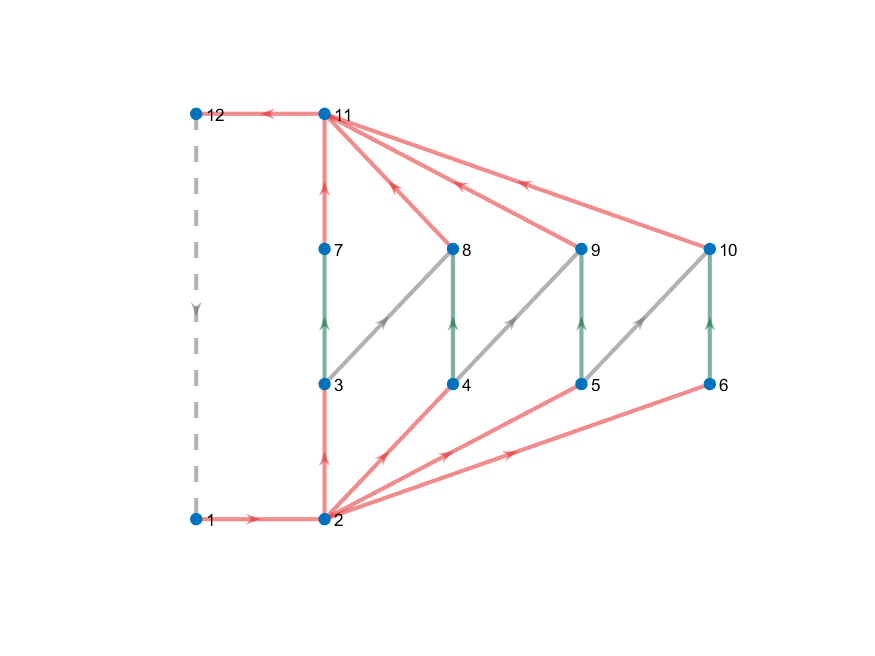
\includegraphics[width=\textwidth]{../attachments/f-dege-mac-4.png}
        \caption{}
        \label{fig:d-size-4}
    \end{subfigure}
    \hspace{0.05\textwidth}
    \begin{subfigure}[b]{0.45\textwidth}
        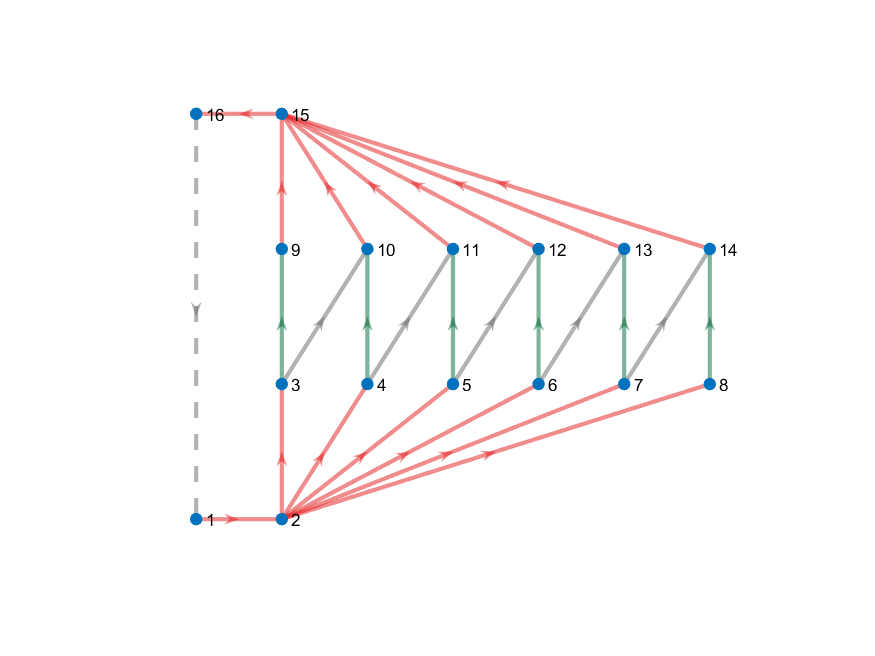
\includegraphics[width=\textwidth]{../attachments/f-dege-mac-6.png}
        \caption{}
        \label{fig:d-size-6}
    \end{subfigure}

    \caption{Results obstained by our method on structure proposed by Visairo\cite{visairoReconfigurableBatteryPack2008} with (a)2, (b)4 and (c) 6 batteries.  The red highlighted lines indicate the open/close states of switches.}
    \label{fig:d-size}
\end{figure}

\begin{table}[h]
    \caption{detailed results of the proposed method for the rbs structure  proposed by visairo\cite{visairoReconfigurableBatteryPack2008} with (a)2, (b)4 and (c) 6 batteries , including the output current, current of each battery, and $\eta$.}
    \label{tab:d-size}
    \begin{tabular}{cccc}
        \hline
        size &  output current $I_o$       & battery current $\bm{I}_b$       & $\eta$        \\
        \hline\\
        2 &  $\displaystyle\frac{2u_b}{2R_o + r_b}$ &  $\displaystyle\left[\frac{u_b}{2R_o + r_b},\frac{u_b}{2R_o + r_b},\frac{u_b}{2R_o + r_b},\frac{u_b}{2R_o + r_b}\right]$   & $2.00$ \\
        \\
        4 &  $\displaystyle\frac{4u_b}{4R_o + r_b}$ &  $\displaystyle\left[\frac{u_b}{4R_o + r_b},\frac{u_b}{4R_o + r_b},\frac{u_b}{4R_o + r_b},\frac{u_b}{4R_o + r_b}\right]$   & $4.00$ \\
        \\
        6 &  $\displaystyle\frac{6u_b}{6R_o + r_b}$ &  $\displaystyle\left[\frac{u_b}{6R_o + r_b},\frac{u_b}{6R_o + r_b},\frac{u_b}{6R_o + r_b},\frac{u_b}{6R_o + r_b}\right]$   & $6.00$ \\
        \\
        \hline
    \end{tabular}
\end{table}

Our greedy algorithm provided accurate estimates of the structure MAC and generated safe and effective switch control strategies, as indicated by the results shown in Figure \ref{fig:d-structure} and \ref{fig:d-size}, where the highlighted red switches denote the closed positions.
Furthermore, the current solutions obtained from the control strategies in Table \ref{tab:d-structure} and \ref{tab:d-size} show that the output current is influenced by the external circuit resistance, battery potential, and internal resistance, but is linearly related to the battery current, consistent with the conclusion about $\eta$ in the previous subsection.

\subsection{Advantages and future improvements}

Our proposed method can obtain comprehensive information about the battery system, including the voltage, current, power, and energy of each battery, as well as the output voltage and current of the system.
This information can be used for various reconfigurable circuit metrics, such as output voltage regulation, power balancing, and fault diagnosis.
By using this method, engineers and researchers can obtain a better understanding of the behavior and performance of battery systems, and optimize their designs and operations accordingly.

To further enhance the usefulness of our method, we can modify the equivalent battery model by introducing capacitance to analyze the transient behavior of the battery system.
This modification can capture the dynamic response of the battery system to sudden changes in load or input voltage, and enable more accurate simulations of battery systems under transient conditions.
By incorporating these models and techniques, we can achieve more accurate and realistic simulations of battery systems, and enable more advanced analysis and design of battery systems.


\section{Conclusion}

In conclusion, we successfully estimated the Maximum Allowable Current (MAC) of the Rechargeable Battery Systems (RBSs), which is an important performance indicator for evaluating the RBSs.
We developed both a graph model and a circuit model and used a greedy strategy to solve the MAC.
Our method was validated for RBS structures of different sizes and configurations, demonstrating its effectiveness for handling complex models in practice.
This work provides an effective approach for designing and evaluating the output current performance of RBS.
Our model can be used to obtain current and voltage information for different nodes and branches, and is scalable for larger systems.
Future work could focus on :
a) using current and voltage information to construct new performance indicators for evaluating RBS performance, and
b) modifying the equivalent model of the battery for circuit model applications, such as transient analysis.


\bibliographystyle{ieeetr}
\bibliography{../attachments/my_ref}

\end{document}
